%
\section{The Fundamentals Behind MultiRegions}

Up to now in the library, the various data structures and methods associated with standard regions, spatial domains and local regions are not 
specifically dictated by any particular numerical method.   In fact, at this stage, they can all be viewed in light of approximation theory.  With
local regions in place, we have a region in world space over which we can represent an expansion (i.e. linear combination of basis functions)
and form its derivatives and its integral.  It is at the level of MultiRegions that we now combine two fundamental concepts: the idea of a collection
of elements together to form a ``global" expansion and the idea of how these (local) elements communicate (in the sense of how does one form
approximations of a PDE of these collections of elements).   Hence MultiRegions is important because it gives us a way of dealing with general tessellation and
also because it is the first place at which we can connect to a specific numerical PDE approximation methods of choice (i.e. continuous Galerkin FEM methods,
discontinuous Galerkin finite volume methods, etc.).

Because MultiRegions is both about grouping of elements in space (to form a domain) and about solving PDEs over these domains, you will find two primary
collections of routines contained within the MultiRegions directory.  You will find things related to collections of elements:  ExpList (Expansion List), DisContField (discontinuous
field) and ConField (continuous field); and you will find objects related to the linear systems formed based upon the particular numerical method once selects (i.e. GlobalLinSys, 
which stands for Global Linear System).

At present, the {\nek} framework supports three types of numerical PDE discretizations for conservation laws:

\begin{itemize}
\item {\bf Discontinuous Galerkin Methods:} These weak-form (variational) methods do not require element continuity, but do put restrictions on the flux of information between elements.  In general, these methods can be thought of as being in the class of finite volume (FV) methods.  One feature of these methods that is often exploited computationally is that
many operations can be considered as elemental.   See \cite{CockburnKS,HesthavenW08} and references therein for a more complete summary.
%
\item {\bf Continuous Galkerin Methods:}  These weak-form (variational) methods require at least $C^0$ continuity.  Mathematically, there have been extensions to 
higher levels of continuity, e.g. Isogeometric Analysis  \cite{CottrellISO}, these are not implemented in {\nek} and would require further constraints on our SpatialDomain
representations than we currently accommodate.  In general, these methods can be thought of as being in the class of finite element methods (FEM).  Although 
these methods are technically (mathematically) formulated as global methods, their elemental construction and compact basis types allow for many local operations.
Many (but not all) of the linear system routines that are contained with the MultiRegions directory are focussed on this discretization type.
See \cite{Schwab, DevilleFM02,KaSh05}  and references therein for a more complete summary.
%
\item {\bf Flux Reconstruction Methods:}  These strong-form methods do not require element continuity, but like dG methods they impose restrictions on the flux of information between elements.  In general, these methods can be though of as being in the class of generalized finite difference (FD) or collocating methods. 
See  \cite{Kopriva,WitherdenVJ2016} and references therein for a more complete summary.
\end{itemize}

\paragraph{Assembly Map}



\begin{figure}[htb]
\centering
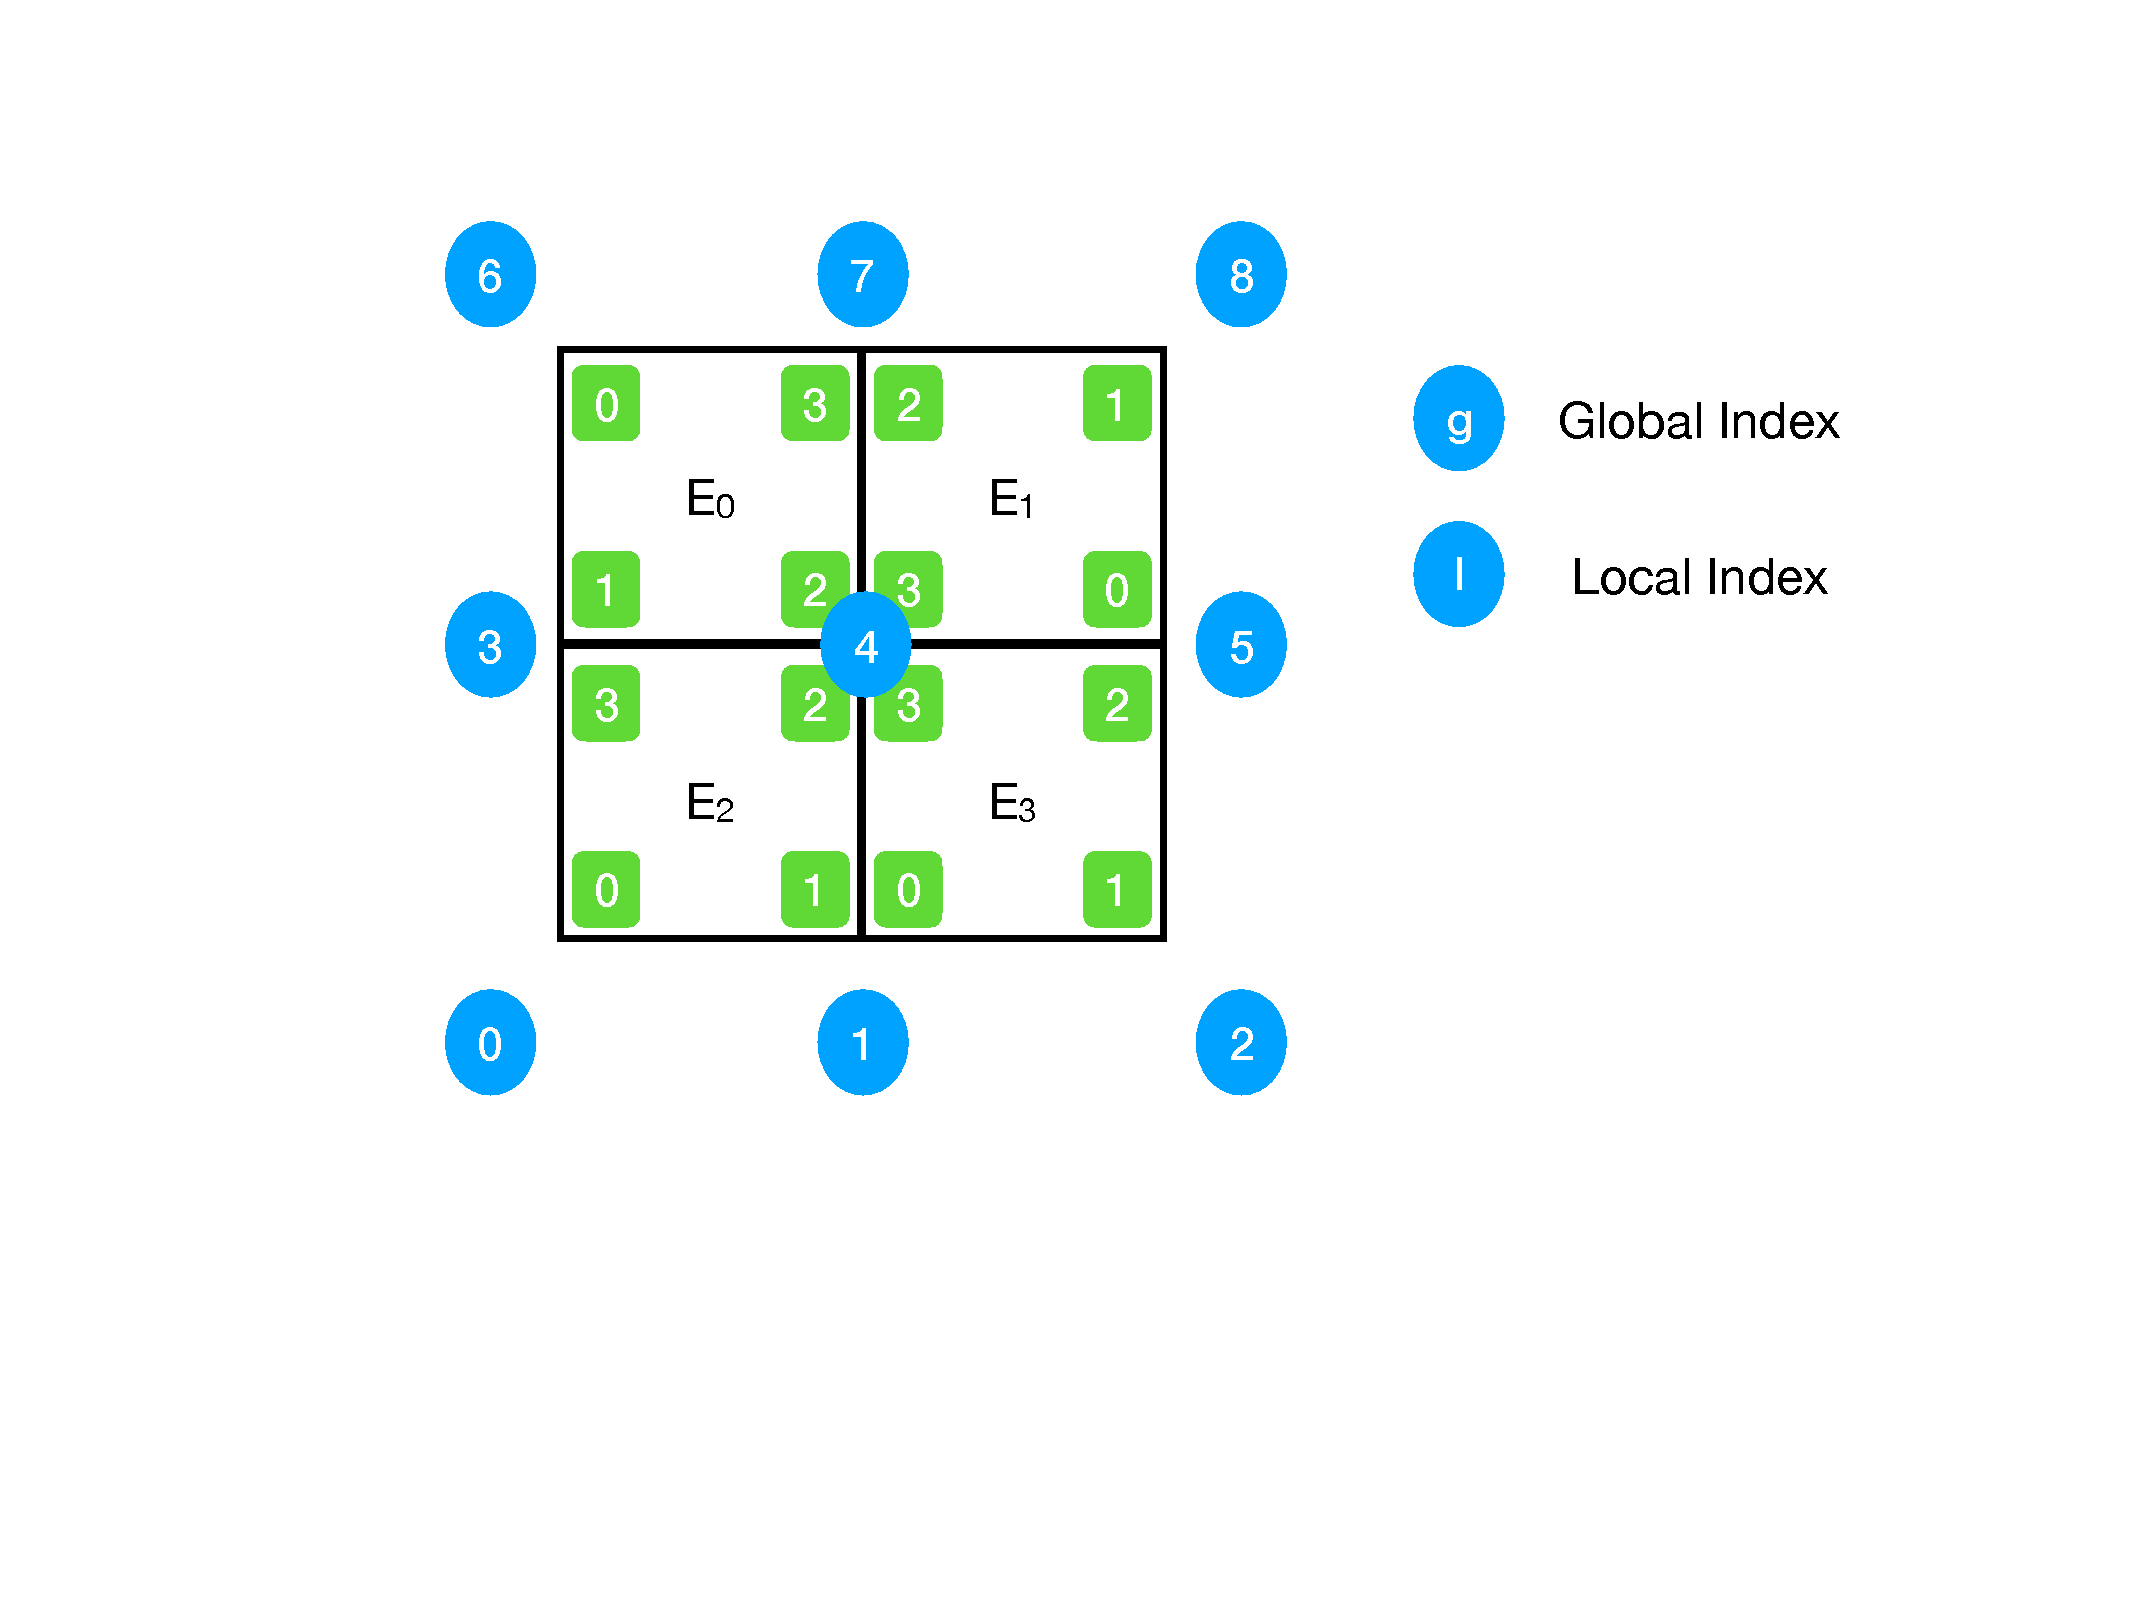
\includegraphics[width=4in]{img/Assembly1.pdf}
\caption{Diagram to help explain assembly.  UPDATE.}
\label{multiregions:assembly1}
\end{figure}


\begin{figure}[htb]
\centering
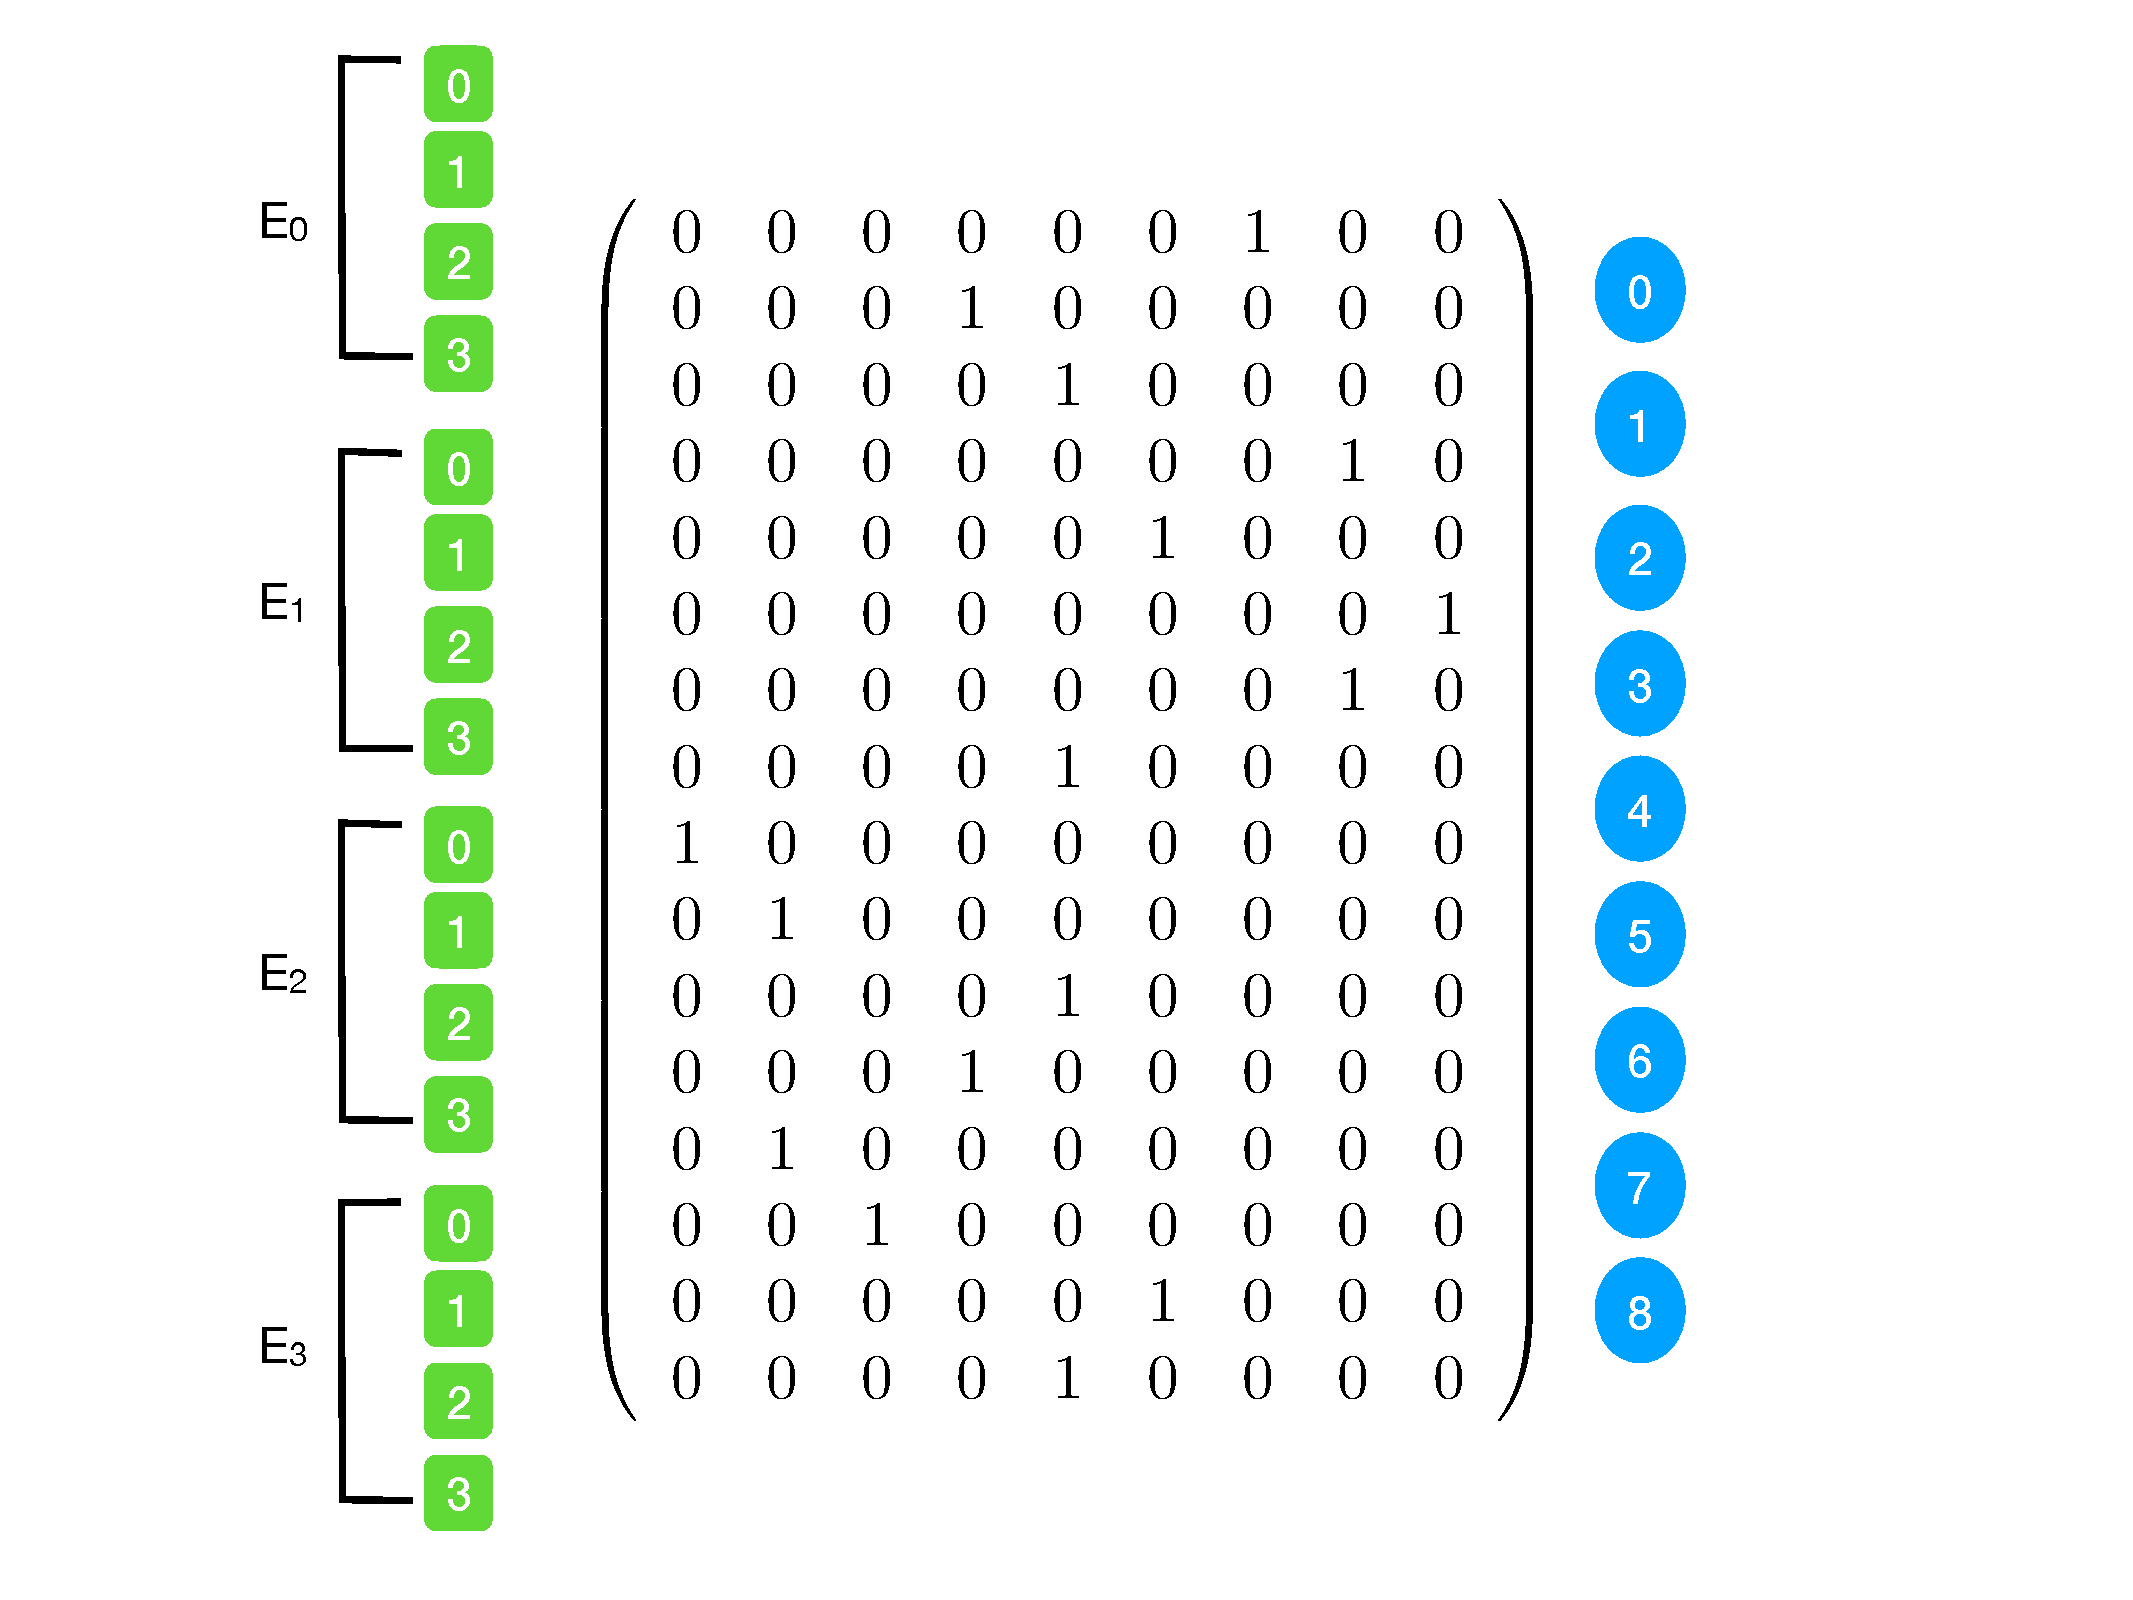
\includegraphics[width=4in]{img/Assembly2.pdf}
\caption{Diagram to help explain assembly.  UPDATE.}
\label{multiregions:assembly2}
\end{figure}

